\documentclass[10pt, landscape, a4paper]{article}
\usepackage{geometry}[landscape]
\usepackage{multicol}
\usepackage{graphicx}
\usepackage{amsmath} 
\usepackage{amssymb}
\usepackage{ccicons}
\usepackage{hyperref}

\usepackage[dvipsnames]{xcolor}

% Set page margins
\geometry{top=.8cm, left=.8cm, right=.8cm, bottom=.8cm}

% Set paragraph indentation
\setlength{\parindent}{0pt}

% Set path for assets
\graphicspath{{assets/}}

\setlength{\columnsep}{20pt}
\raggedcolumns

% _____ CUSTOM COMMANDS __________________________________________
\newcommand{\E}[0]{\mathbb{E}}
\newcommand{\R}[0]{\mathbb{R}}

\newcommand{\sgn}[0]{\text{sgn}}

\newcommand{\argmin}[1]{\underset{#1}{\text{argmin}}}
\newcommand{\argmax}[1]{\underset{#1}{\text{argmax}}}

\begin{document}
\begin{multicols*}{3}

% _____ CONTENT __________________________________________________

% main heading
\begin{center}
	\Large{\textbf{Visual Computing}} \\
    \small{by dcamenisch}
\end{center}

\section{Introduction}

This document is a summary of the 2022 edition of the lecture \textit{Visual Computing} at ETH Zurich. I do not guarantee correctness or completeness, nor is this document endorsed by the lecturers. If you spot any mistakes or find other improvements, feel free to open a pull request at \url{https://github.com/DannyCamenisch/vc-summary}. This work is published as CC BY-NC-SA.
\begin{center}
	\ccbyncsa
\end{center}
\section{The Digital Image}

An image is simply a continuous function over 2 or 3 variables (XY-coordinates and possibly time). Usually we use brightness as the value of the function, but other physical values can also be used. For a computer this is just a collection of numbers, but instead of continuous values we have discrete. Note that in real life images are never completely random and almost always contain some structure. It is important to know that \textbf{pixels are not little squares}, they are point measurements.

When taking a picture with a digital camera, we can encounter various problems, e.g.:
\begin{itemize}
	\item Transmission Interference
	\item Compression Artefacts
	\item Spilling
	\item Sensor Noise
\end{itemize}

\subsection{Sampling}

When taking an image, we are sampling such a continuous. When trying to reconstruct the original function, we can encounter undersampling, i.e. when we loose information due to a too low amount of sampling points. 

\begin{center}
	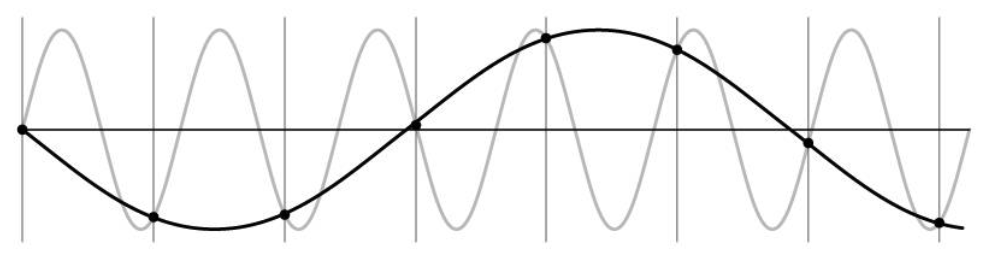
\includegraphics[width=0.8\linewidth]{undersampling.png}
\end{center}

Due to undersampling, the result can not be distinguished from a lower or a higher frequency wave. Signal disguised as other frequencies is also called \textbf{aliasing}. \medskip

\textbf{Nyquist-Shannon Sampling Theorem}

For sine waves we have to sample at half the wave length. This corresponds to double the frequency, we also call this the \textbf{Nyquist Frequency}.

\subsection{Quantization}

Another problem we have to deal with is \textbf{quantization}, since the real valued function will get digital (integer) values, it is lossy. Compared to sampling which lets us reconstruct the original function. Simple quantization uses equally spaced levels with $k$ intervals.

\begin{center}
	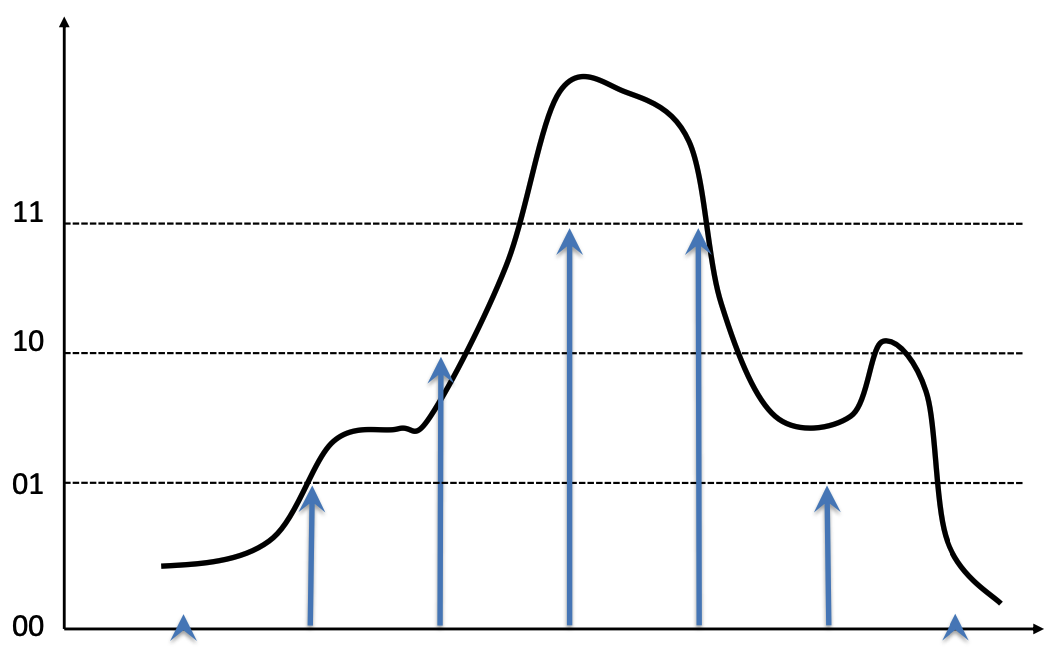
\includegraphics[width=0.8\linewidth]{quantization.png}
\end{center}

\subsection{Image Properties}

Image resolution is divided into two parts:
\begin{itemize}
	\item Geometric Resolution: How many pixels per area
	\item Radiometric Resolution: How many bits per pixel
\end{itemize}

\subsection{Noise}

When taking pictures we can almost always encounter some noise. A common way to model this is additive gaussian noise:
$$I(x,y) = f(x,y) + c, \qquad c \sim \mathcal N(0, \sigma^2)$$

The signal to noise ratio (SNR) is an index of image quality:
$$\text{SNR} = \frac{F}{\sigma}, \qquad F = \frac{1}{XY} \sum_{x=1}^{X}\sum_{y=1}^{Y} f(x,y)$$

The usefulness for this metric can vary drastically depending on the type of image (dark images will have a higher SNR compared to bright images). Therefore we introduce peak SNR:
$$\text{PSNR} = \frac{F_\text{max}}{\sigma}$$
\section{Segmentation}

Image segmentation is often viewed as the ultimate classification problem, once solved, computer vision is solved. A complete segmentation of an image is a finite set of disjunct regions $R_1, ..., R_n$, such that $I = \bigcup R_i$.


\subsection{Thresholding}

Thresholding is a simple segmentation process, that produces a binary image by labelling each pixel in or out of the region of interest. We do this by comparison of the grey level with a threshold value $T$. Another, better approach can be chromakeying. Hereby we measure the distance from a defined color $g$:

$$I_\alpha = |I - g| > T$$

One limit of thresholding is that it does not consider image context.


\subsection{Segmentation Performance}

If we want to choose the best performing segmentation algorithm or determine a good value for $T$, we need a performance metric. To use automatic analysis, one needs to know the true classification of each test, for this the test images have to be segmented by hand. \medskip

One performance metric is the ROC curve. This curve characterizes the error trade-off in binary classification tasks, by plotting the true positive fraction against the false positive fraction. We often choose the operating point on the ROC curve, by assigning cost and values to each outcome:
\begin{itemize}
	\item $V_{\text{TN}}$ - value of true negative
	\item $V_{\text{TP}}$ - value of true positive
	\item $C_{\text{FN}}$ - cost of false negative
	\item $C_{\text{FP}}$ - cost of false positive
\end{itemize}

We then choose the point on the ROC curve with the gradient:
$$\beta = \frac{N}{P} \cdot \frac{V_{\text{TN}} + C_{\text{FP}}}{V_{\text{TP}} + C_{\text{FN}}}$$


\subsection{Pixel Connectivity}

We try to define which pixels are neighbors.

\begin{center}
	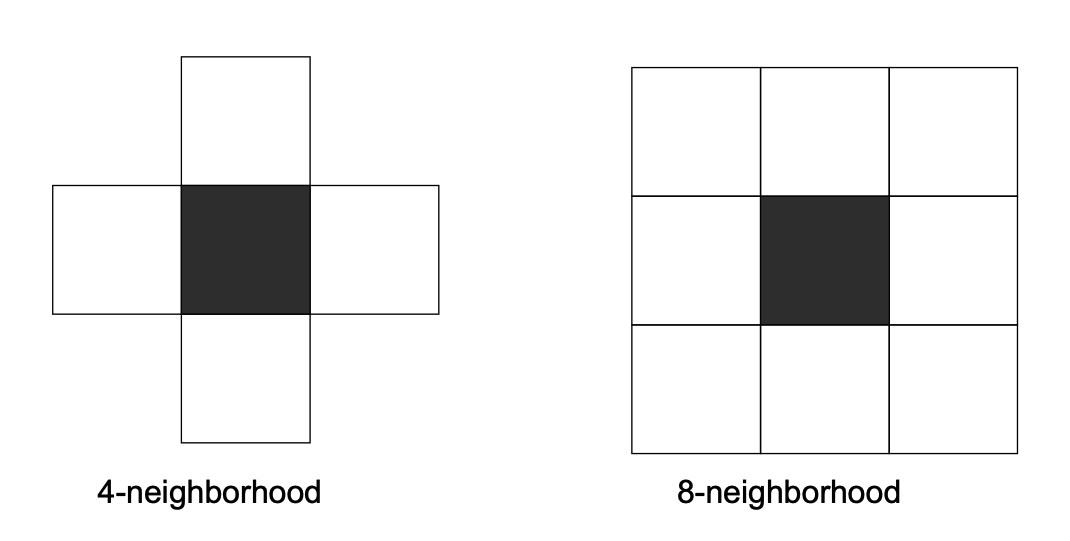
\includegraphics[width=\linewidth]{pixel-neighborhoods.png}
\end{center}

A 4 (or 8) connected path between $p_1, p_n$ is a set of pixels such that every $p_i$ is a 4 (or 8) neighbor of $p_{i+1}$. Now we can defined a region as 4 (or 8) connected if it contains a 4 (or 8) connected path between any two of its pixels.

With this we can introduce \textbf{region growing}. We start from a seed point or region and add neighboring pixels that satisfy the criteria defining a region until we can include no more pixels. There are different approaches to selecting the seed and we could also use multiple seeds. For the inclusion criteria we could choose thresholding or a distribution model.

Another criteria is a snake (active contour). While each point along the contour moves away from the seed, it always has to have some smoothness constraints (minimizing energy function).


\subsection{Distance Measures}

Plain background substraction $I_\alpha = |I - I_{bg}| > T$, where $I_{bg}$ is the background image, we get this by fitting a Gaussian (Mixture) model per pixel. Even better would be:
$$I_\alpha = \sqrt{(I - I_{bg})^\top \Sigma (I - I_{bg})} > T$$

Where $\Sigma$ is the background pixel appearance covariance matrix.


\subsection{Markov Random Fields}

We can add spatial relations with Markov Random Fields (2D Markov Chains).

\begin{center}
	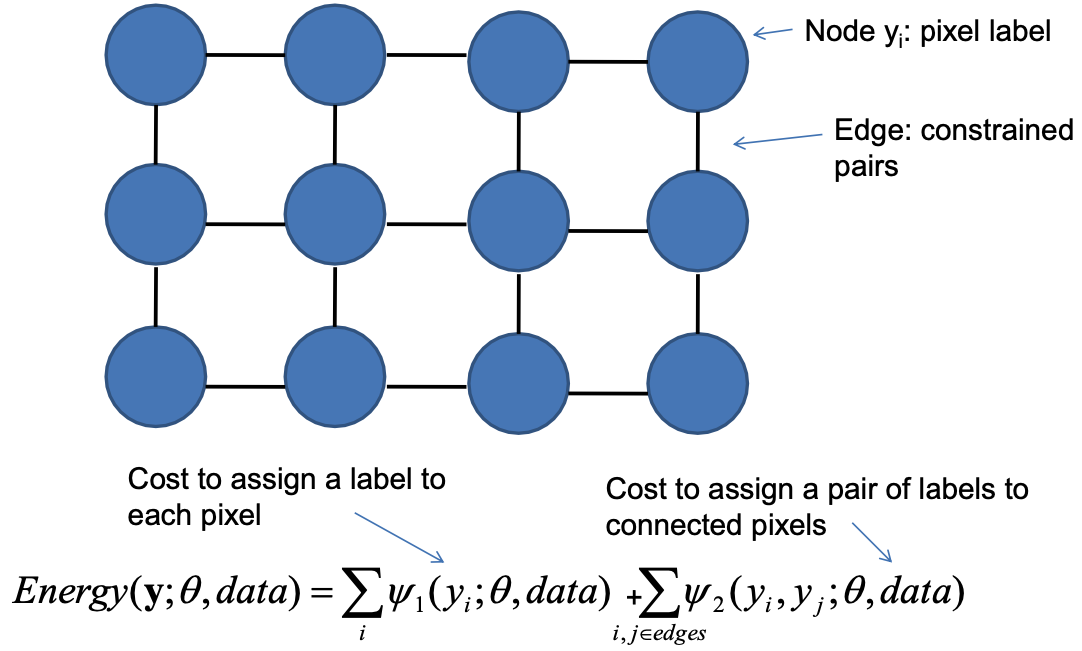
\includegraphics[width=\linewidth]{markov-field.png}
\end{center}

Using a graph cut algorithm we can determine the optimal segementation. We can further optimize this by using iterated graph cut and k-means for learning the colour distribution (GMM) of the image.

\begin{center}
	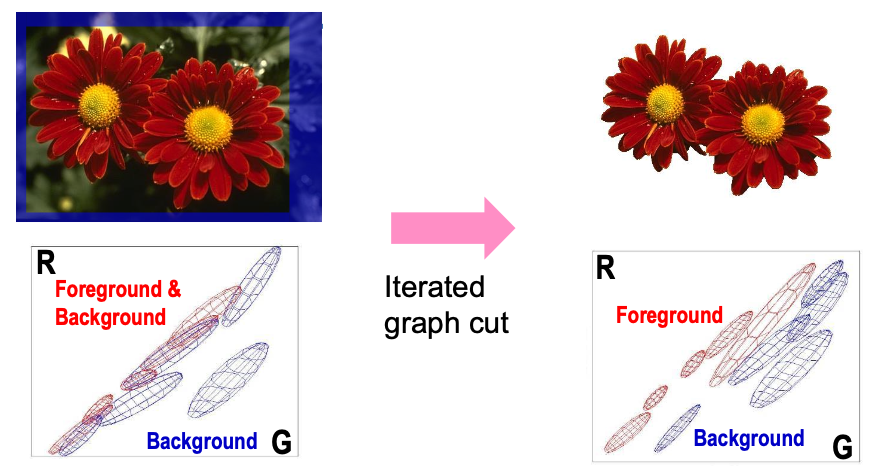
\includegraphics[width=\linewidth]{iterated-graph-cut.png}
\end{center}

\section{Convolution and Filtering}

Convolution and filtering are some of the most basic operations of image processing. 


\subsection{Filtering}

Image filtering is the process of modifying pixels in an image base on some function of a local neighborhood of the pixel.

\subsubsection{Linear Shift-Invariant Filtering}

Linear lhift-invariant filtering means using linear combinations of neighbors and doing the same for each pixel (shift-invariant). These filters are often used for low-level image processing, smoothing / noise reduction, sharpening and feature detection. Linear operations can be written as:
$$I'(x,y) = \sum_{(i,j) \in N(x,y)} K(x,y; i, j) I(x,y)$$

Here $I$ is the input image, $I'$ the output image, $K$ is the kernel and $N$ is the neighborhood. Operations are shift-invariant if $K$ does not depend on $(x,y)$.


\subsection{Correlation}

Correlation, e.g. template matching:

\begin{center}
	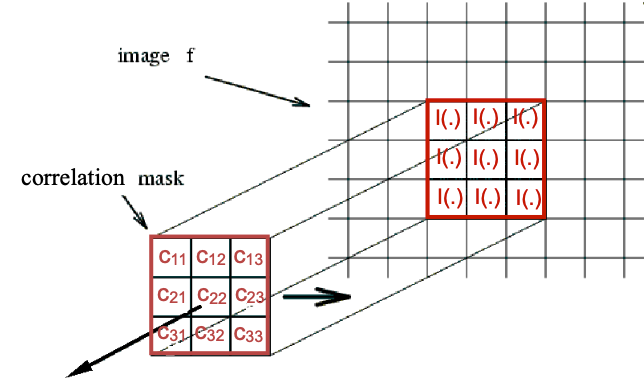
\includegraphics[width=0.9\linewidth]{correlation.png}
\end{center}
$$I' = K \circ I, \quad I'(x,y) = \sum_{(i,j) \in N(x,y)} K(i, j) I(x + i, y + j)$$

Correlation takes an input image and a weight mask, then each pixel gets "replaced" by the weighted sum of its neighborhood. This can be described as taking multiple input location and writing one output location.


\subsection{Convolution}

Convolution, e.g. point spread function:

\begin{center}
	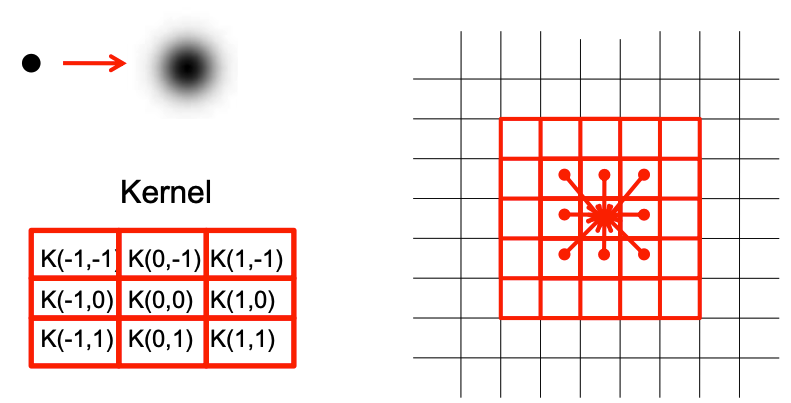
\includegraphics[width=0.9\linewidth]{convolution.png}
\end{center}
$$I' = K * I, \quad I'(x,y) = \sum_{(i,j) \in N(x,y)} K(i, j) I(x - i, y - j)$$

This is similar to the correlation, but \textbf{the kernel is reversed}. This can be described as taking one input location and writing multiple output location, the opposite of the correlation. By default we use convolution for filtering. An example for a kernel would be:
$$ K = 
\begin{bmatrix}
    0 & 0 & 0\\
    0 & 2 & 0\\
    0 & 0 & 0
\end{bmatrix}
 -
\frac{1}{9}
\begin{bmatrix}
   1 & 1 & 1\\
   1 & 1 & 1\\
   1 & 1 & 1
\end{bmatrix}
$$

This kernel is used for sharpening by accentuating differences with the local average. Another example would be:
$$ K = 
\begin{bmatrix}
    -1 & 0 & 1\\
    -2 & 0 & 2\\
    -1 & 0 & 1
\end{bmatrix}
$$

This kernel looks for differences in the horizontal direction, this corresponds to finding vertical edges.

\subsubsection{What about the Edges?}

If we apply our filters to images, we need to \textbf{deal with the edges separately}. This is due to our window falling off the edge of the image. There are different techniques to deal with this problem:
\begin{itemize}
	\item Extend the image with black border
	\item Wrap the kernel around the edges
	\item Copy out the edge
	\item Mirror the image at the edge
	\item Vary filter near the edge
\end{itemize}

\subsubsection{Separable Kernels}

A kernel is separable, if it can be written as $K(m, n) = f(m) g(n)$. This means that the kernel can be separated into a function for the first coordinate and another for the second coordinate. If this is the case we can apply the separated functions individually to the image.

\subsubsection{Gaussian Kernel}

The idea of the \textbf{Gaussian Kernel} is to weight the contributions of neighboring pixels by nearness.

\begin{center}
	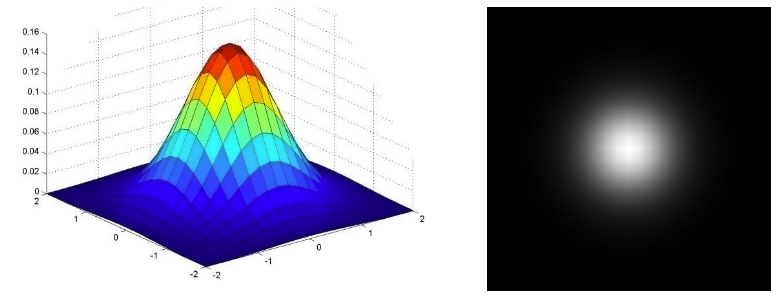
\includegraphics[width=0.9\linewidth]{gaussian_kernel.png}
\end{center}
$$G_\sigma = \frac{1}{2 \pi \sigma^2}^{- \frac{(x^2 + y^2)}{2 \sigma^2}}$$

We can use the Gaussian Kernel for image smoothing, the best part being that the kernel is separable. The actual amount of smoothing depends on $\sigma$ and the window size. \medskip

If we repeatedly apply the Gaussian filter, we produce the scale space of an image.

\subsubsection{High-Pass Filters}

High-pass filters are used to detect areas of the image where a lot is happening (high frequencies). Examples for these are the Laplacian operator $K$ or the high-pass filter $K'$:
$$ K = 
\begin{bmatrix}
    0 & 1 & 0\\
    1 & -1 & 1\\
    0 & 1 & 0
\end{bmatrix}
\qquad
K' =
\begin{bmatrix}
    -1 & -1 & -1\\
    -1 & 8 & -1\\
    -1 & -1 & -1
\end{bmatrix}
$$

High-pass filters can be used to perform image sharpening $I' = I + \alpha |K * I|$.


\end{multicols*}
\end{document}

% ____ FOOTER ______________________________________________________
% Content and Template: 
% original by Danny Camenisch (dcamenisch@inf.ethz.ch), 2022
% based on different summaries from many helpful people